\scanpage{110}
% Archive foliation: 111.
\[
0\longrightarrow N-G\xrightarrow{u}H\longrightarrow0\quad\not\Longrightarrow\quad\overset{\text{\inserted{\figure{\begin{tikzpicture}\node[draw,ellipse] {\unsure{formellt}};\end{tikzpicture}}}}}{\text{\uline{ker est lisse}}}
\]
\deleted{$G(\hat S)\longrightarrow H(\hat S)$}

$G\longrightarrow H$

$\Phi(G)\longrightarrow\Phi(H)$ \uline{surj.}

$G\xrightarrow{u}H$\qquad hom de gpes divisibles \unsure{sur le T.K.}

Conditions équivalentes

(i) L'hom $u(1):G(1)-H(1)$ est un \uline{épim.}
\margin{[il suffit de vérifier sur fibre spéciale]}

(ii) L'hom $u(n):G(n)-H(n)$ est un [idem] épim $\forall n$.

(iii) L'hom $u$ est \uline{formellt lisse} et un \uline{épim.}

(iii bis) L'hom $u_s:G_s-H_s$ est form\textsuperscript{t} lisse et un épim.

(iv) L'hom de gpes divisibles sur $K$ :
\[
G_{|K}-H_{|K}
\]
\deleted{\unsure{est un}} [form\textsuperscript{t} lisse et] un épim

(iv bis) $\Phi(G)-\Phi(H)$ est surjectif

\figure{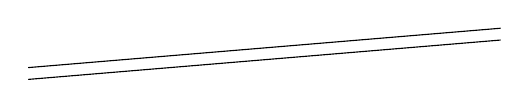
\begin{tikzpicture}\draw(0,0)--(6,.5);\draw(0,-.15)--(6,.35);\end{tikzpicture}}

\diagram{\left\{\begin{array}{ll}
a)&\text{Si }\Phi(u)\text{ est un isom, alors }u\text{ est un isom}\\
&\text{($\Phi$ est ``conservatif'')}\\
b)&\text{Si }u\text{ est déjà formellt fid. plat, }\deleted{\unsure{\Phi(u)\text{ surj}}}\\
&\text{mais pas form\textsuperscript{t} lisse [i.e. Ker }u\text{ pas form\textsuperscript{t} lisse]}\\
&\text{alors }\Phi(u)\text{ pas surjectif}\ldots
\end{array}\right.}
